\documentclass{article}

% NeurIPS/ICML style packages
\usepackage[final]{icml_2024} % Use neurips style (can be replaced with icml style)
\usepackage{natbib}
% \bibliographystyle{unsrt}   % Numbers in citation order


\usepackage{graphicx}
\usepackage{amsmath}
\usepackage{mathtools}
\usepackage{amssymb}
\usepackage{tikz}
\usetikzlibrary{arrows.meta, positioning, shapes, fit}
% \usepackage{algorithm}
% \usepackage{algpseudocode}
\usepackage{hyperref}
\usepackage{url}
\usepackage{booktabs}
\usepackage{microtype}

% \usepackage[ruled, vlined, linesnumbered]{algorithm2e}

\newcommand{\ak}[1]{\textcolor{red}{ak: #1}}
\newcommand{\bk}[1]{\textcolor{blue}{: #1}}


% Theorem environments
\usepackage{amsthm}
\newtheorem{theorem}{Theorem}
\newtheorem{lemma}[theorem]{Lemma}
\newtheorem{proposition}[theorem]{Proposition}
\newtheorem{corollary}[theorem]{Corollary}
\newtheorem{definition}{Definition}
\newtheorem{example}{Example}
\newtheorem*{example*}{Example}
\newtheorem{remark}{Remark}
\newtheorem{claim}{Claim}
\newtheorem{note}{Note}

\title{Distributional Rewards in MDPs}

% \author{
%   Author One\thanks{Equal contribution.} \\
%   Department of Computer Science\\
%   University Name\\
%   \texttt{author1@university.edu} \\
%   \And
%   Author Two\footnotemark[1] \\
%   Department of Computer Science\\
%   University Name\\
%   \texttt{author2@university.edu} \\
% }

\begin{document}

\maketitle

\begin{abstract}
Classical Markov Decision Processes (MDPs) suffer from exponential state-space growth in multi-agent systems. Recent work on distributional MDPs addresses this challenge by tracking agent distributions rather than individual states, successfully handling qualitative objectives such as safety and reachability. However, we are also interested in optimizing quantitative performance metrics. Traditional MDPs employ state-based reward functions, yet in multi-agent systems, meaningful rewards often depend on the collective distribution of agents rather than individual states.

We introduce distributional reward functions that assign rewards based on the collective agent distribution, enabling the expression of congestion penalties, formation quality metrics, load balancing objectives, and other aggregate performance measures. We develop a value iteration algorithm for computing optimal deterministic distributional policies under structured reward functions by representing value functions as maxima over finite vector sets. For the infinite-horizon setting, we establish existence and uniqueness of optimal value functions via contraction mapping arguments, proving geometric convergence of value iteration.
\end{abstract}

\section{Introduction}

Classical Markov Decision Processes (MDPs) have been successful for modeling sequential decision-making in single-agent systems. However, when we move to multi-agent settings, the classical state-based approach encounters a fundamental computational barrier: the state space grows exponentially with the number of agents. Consider $m$ identical robots navigating an $n \times n$ grid—the state space has size $n^{2m}$, which becomes intractable even for modest swarm sizes. This exponential growth is not merely a computational inconvenience; it represents a fundamental mismatch between how we represent the system and what information we actually care about.

\textbf{The Distributional Perspective.} In many multi-agent scenarios, the identity of individual agents is irrelevant—what matters is the collective behavior. Do we really need to know that robot \#47 is at position $(3,5)$? Or do we only care that 15\% of the robots are at position $(3,5)$? This distributional perspective, introduced in ~\citep{akshay2018distributionbased} and developed further in~\citep{akshay2023mdpsdistributiontransformersaffine, akshay2024certifiedpolicyverificationsynthesis}, tracks the \emph{distribution} of agents across states rather than individual agent positions. This distributional representation has dimension $|S|$—completely independent of the number of agents—providing exponential compression. Moreover, distributional strategies can condition on global information (like "what fraction of agents have reached the goal?") that individual agents cannot access.



\textbf{Prior Work.} The distributional perspective for MDPs, where system evolution is tracked as probability distributions over states rather than individual trajectories, was introduced in ~\citep{akshay2018distributionbased}. These distributional properties are computationally hard—Skolem-hard for reachability~\citep{akshay2015reachability}

% and inexpressible in standard temporal logics~\citep{beauquier2006logic}.

Recent work has successfully synthesized ( with semi-completeness guarantees )  distributional strategies for \emph{qualitative} specifications~\citep{akshay2023mdpsdistributiontransformersaffine, akshay2024certifiedpolicyverificationsynthesis}: safety objectives (maintaining distributions within safe sets) and reachability objectives (reaching target sets). The framework of~\citep{akshay2023mdpsdistributiontransformersaffine} uses affine invariants and template-based synthesis, while~\citep{akshay2024certifiedpolicyverificationsynthesis} extends this to reach-avoidance properties with certified synthesis procedures.


% I have cited them later in related work - no it has to be here too.
% \ak{read the intro and related work sections of these two papers, and then see which prior work need to be cited and add them.}

Now that multi-agent systems can be modeled using the distributional view of MDPs ,
% \ak{add original refs also -- see comment in intro} % I couldnt the find orginal ref
we also wish to optimize performance metrics, typically formulated as rewards. In this setting, traditional state-based rewards are insufficient, as they cannot capture many reward structures that arise naturally in multi-agent system as a state-based reward of the form $R(s,a,s')$ depends only on the local transition and does not depend on the global distribution at that time step.

We now present an example where state-based rewards cannot be used, at least not in a simple or natural manner, to capture the desired objective. 

\begin{example*} \label{example1}
    Consider a warehouse floor consisting of storage cells, pathways, and packing stations. A large swarm of robots transports items to their final destinations. Our goal is to minimize the total time taken while also reducing congestion at each grid cell as the robots move.
\end{example*}
 We can model this system using the distributional view of MDPs. However, using state-based rewards fails to provide an appropriate formulation. Since a state-based reward assigns a value only to a single state transition, it cannot capture congestion effects. To penalize congestion (i.e., when more than an optimal number of robots occupy the same cell), we must know how many other robots are present in that cell, which is not available in the traditional reward framework. 

In light of the above problems , In this paper we introduce a new type of reward function which depends on the entire global distribution which helps us formulate the reward functions arising in the multi-agent systems .

\textbf{Contributions.} 
Our main contributions are:\begin{enumerate}

    \item We introduce  \textbf{ \emph{distributional reward functions} } $R_{\text{dist}}: \Delta(S) \times \Delta(A)^{|S|} \to \mathbb{R}$ that assign rewards based on the current distribution and action selections. This strictly generalizes classical rewards 
    % \ak{do you have a proof of this?}-> done below 
    and enables expressing congestion penalties, formation quality metrics, and load balancing objectives. 

% \ak{great, but each of these should be explained somewhere using examples, either using the motivating example above or in sec 3 $->$ Will explain each of them in the following examples , still trying to get some realistic examples }
    
    \item  We develop a \textbf{ value iteration algorithm } for getting optimal  deterministic policy (Section~\ref{sec:value-iteration}) for finite and infinite horizon cases .
    
 % \ak{what is the novelty/difficulty here? -> difficulty explained in the value iteation section }
 
\end{enumerate}

\subsection{Related Work}

\textbf{Distributional MDPs.} The view of MDPs as distribution transformers, where the system state is represented as a probability distribution evolving over time, was introduced by~\citep{akshay2018distributionbased}. This perspective is particularly natural for modeling multi-agent systems, chemical reaction networks, and population protocols, where individual identities are irrelevant and only aggregate behavior matters. Early work by~\citep{kwon2011verifying} introduced the iLTL logic for reasoning about probability mass functions in DTMCs, while~\citep{chadha2011model} studied MDPs with unique compact invariant sets of distributions.

\textbf{Computational Hardness.} The verification and synthesis problems for distributional properties are computationally challenging.~\citep{akshay2015reachability} showed that distributional reachability is as hard as the Skolem problem, a long-standing open problem in number theory whose decidability remains unknown~\citep{ouaknine2012decision}. Furthermore,~\citep{beauquier2006logic} demonstrated that distributional properties such as reachability and safety cannot be expressed in PCTL*, rendering classical probabilistic model checking techniques inapplicable.

\textbf{Distributional Synthesis for Qualitative Objectives.} Recent work has developed synthesis methods for qualitative distributional specifications.~\citep{akshay2023mdpsdistributiontransformersaffine} introduced affine invariant synthesis for distributional safety objectives, showing that even simple MDPs may require infinite memory and randomization for distributional safety. This work was extended by~\citep{akshay2024certifiedpolicyverificationsynthesis} to handle distributional reach-avoidance properties, introducing the notion of distributional reach-avoid certificates and automated synthesis procedures. Both works employ template-based synthesis approaches~\citep{DBLP:journals/corr/abs-1902-04373,Coln2003LinearIG} and provide soundness and relative completeness guarantees.

\textbf{Interpretations of Probability.} The chance-based and mass-based interpretations of probability provide two distinct philosophical frameworks for understanding probabilistic systems~\citep{tsai2025chancemassinterpretationsprobabilities}. The mass-based view, which describes distributions of probability mass across outcomes, aligns naturally with our distributional perspective on multi-agent systems.

\textbf{Value Iteration for POMDPs.} Our algorithmic approach draws inspiration from value iteration methods for Partially Observable MDPs (POMDPs)~\citep{smallwood1973optimal, Krishnamurthy_2016}, which similarly operate over belief spaces (probability distributions over states). However, the distributional MDP setting presents distinct challenges due to the global nature of distributional rewards.

\textbf{Classical MDPs with Rewards.} Foundational work on MDPs with expected rewards~\citep{puterman1994markov, bertsekas1995dynamic} established the Bellman optimality equation and value iteration algorithms for finite state spaces. We extend these classical results to the distributional setting, proving existence and uniqueness of optimal value functions via contraction mapping arguments.


\section{Preliminaries}\label{sec:prelim}
% \ak{add text throughout between definitions. see other papers.}

\begin{definition}[Markov Decision Process(MDP)]
An MDP is a tuple $(S, A, T, \gamma)$ where $S$ is a finite set of states, $A$ is a finite set of actions, $T: S \times A \times S \to [0,1]$ satisfies $\sum_{s'} T(s,a,s') = 1$, and $\gamma \in (0,1)$ is the discount factor .
\end{definition}
    
$\Delta(S) = \left\{ \mu: S \to [0,1] \,\Big|\, \sum_{s \in S} \mu(s) = 1 \right\}$ 


$\Delta(A) = \left\{ \mu: A \to [0,1] \,\Big|\, \sum_{a \in A} \mu(a) = 1 \right\}$

\textbf{State Based View of MDP} : In this view the system evolves as $s_0,s_1,s_2,.. $ where $s_0$ represents the initial state , $s_t$ represents the state of system at time t .

\textbf{Policies in State based view} : At each timestep t , the system is in exactly one state $s_t$ . The action taken at time t can depend on the entire past history of process,i.e $(s_0,a_0,s_1,a_1,..s_t)$ ,
So in full generality, a policy is a function that maps the available history to a probability distribution over actions 

 $\pi_t$ : $H_T \to \Delta(A) $ , where $H_T = (s_0,a_0,s_1,a_1,...s_t) $

A policy is called is called memory less if action at time step t just depends on $s_t$ , $\pi:S \to \Delta(A) $ . A policy is called deterministic if it takes exactly one action for each time step.

Another view to look at MDP is the \textbf{distributional view} Which uses mass based of view of probability instead of chance based view of probability , ( chance and mass based view of probability can be better understood from the paper \citep{tsai2025chancemassinterpretationsprobabilities} ) .


Instead of tracking a single realized trajectory of states $(s_0,s_1,s_2,..)$ , we can describe the system at each time step by a probability mass over states evolving over time .  In the view, system evolves as $\mu_0,\mu_1,\mu_2,..$ , where $\mu_t \in \Delta(S) $ . Here $\mu_0$ is the initial distribution and $\mu_t$ is distribution evolved at time t .

The Distributional Evolution happens as follows :
Given distribution $\mu_t$ and policy $\pi_t: S \to \Delta(A)$, the next distribution is:
$\mu_{t+1}(s') = \sum_{s \in S} \mu_t(s) \sum_{a \in A} \pi_t(s,a) \, T(s,a,s')$.
Equivalently: $\mu_{t+1} = T_\pi^\top \mu_t$ where $[T_\pi]_{ss'} = \sum_a \pi_t(s,a) T(s,a,s')$.



Policies in this view can be similarly both history-dependent and memory-less .

General \textbf{History Dependent Policy} is as follows $$\pi_t : H_t \to \Delta(A)^{|S|}$$ ,$\pi_t(s,a)$ is probability of taking action a at state s ,at time step t .

\begin{note}
We assume that at each time $t$, probability mass is distributed over all states and each portion of that mass takes actions according to the policy. This is different from the normal state-based view where the entire probability mass is in a single state. For example: $P_t(s_1 \text{ is observed at time } t) = P_t(\text{entire prob mass is in } s_1) = 0.4$ in the state-based view, in contrast to $\mu_t(s_1) = 0.4$ in the distributional view where 40\% of the mass is at $s_1$.
\end{note} 

Similarly we can define memory-less policy as the one which just depends on present distribution to generate the action distributions ,$\pi : \mu \to \Delta(A)^{|S|}$ .Similarly deterministic policy is in this setting is taking exactly one action at each state , means $\exists a $ such that $p(s,a) = 1 \quad \forall s$ 


\subsection{Value Functions and Bellman Operators}

Value functions quantify the expected cumulative reward starting from a given state (or distribution) and following a particular policy. They are central to analyzing and solving MDPs.

\begin{definition}[Value Function for State-Based MDPs]
Given a policy $\pi$ and a reward function $R: S \times A \times S \to \mathbb{R}$, the value function $V^\pi: S \to \mathbb{R}$ is defined as:
$$V^\pi(s) = \mathbb{E}\left[\sum_{t=0}^{\infty} \gamma^t R(s_t, a_t, s_{t+1}) \,\Big|\, s_0 = s, \pi\right]$$
where the expectation is taken over the randomness in the policy and transitions.
\end{definition}

The \emph{optimal value function} $V^*: S \to \mathbb{R}$ is:
$$V^*(s) = \sup_{\pi} V^\pi(s)$$

The Bellman optimality equation states that $V^*$ satisfies:
$$V^*(s) = \max_{a \in A} \left[\sum_{s' \in S} T(s,a,s')\left(R(s,a,s') + \gamma V^*(s')\right)\right]$$

\begin{definition}[Bellman Operator]
The Bellman operator $\mathcal{T}: \mathbb{R}^{|S|} \to \mathbb{R}^{|S|}$ is defined as:
$$(\mathcal{T}V)(s) = \max_{a \in A} \left[\sum_{s' \in S} T(s,a,s')\left(R(s,a,s') + \gamma V(s')\right)\right]$$
\end{definition}

The Bellman operator has several important properties:

\textbf{Monotonicity.} If $V_1(s) \leq V_2(s)$ for all $s \in S$, then $(\mathcal{T}V_1)(s) \leq (\mathcal{T}V_2)(s)$ for all $s \in S$.

\textbf{Contraction.} Under the supremum norm $\|V\|_\infty = \max_{s \in S} |V(s)|$, the Bellman operator is a $\gamma$-contraction:
$$\|\mathcal{T}V_1 - \mathcal{T}V_2\|_\infty \leq \gamma \|V_1 - V_2\|_\infty$$

By the Banach fixed point theorem, the contraction property implies that $\mathcal{T}$ has a unique fixed point, and this fixed point is precisely the optimal value function $V^*$. Moreover, the sequence $V_{k+1} = \mathcal{T}V_k$ converges to $V^*$ for any initial $V_0$, forming the basis of the value iteration algorithm.

\textbf{Value Iteration Algorithm.} Value iteration~\citep{bellman1957dynamic, puterman1994markov} is a fundamental dynamic programming algorithm for computing optimal policies in MDPs. Starting from an arbitrary initial value function $V_0$ (typically $V_0 = 0$), the algorithm iteratively applies the Bellman operator: $V_{k+1} = \mathcal{T}V_k$. Due to the contraction property, this sequence converges geometrically to the optimal value function $V^*$. Once $V^*$ is obtained (or sufficiently approximated), the optimal policy can be extracted by choosing actions that achieve the maximum in the Bellman equation.


% \ak{above is good, but also write what in 1-2 slides what VI algo does. why its useful and cite some basic book for it. }

% \ak{then say that our goal is to lift this to distributional setting which we do now.}

\subsection{Lifting to the Distributional Setting}

Our goal is to extend the value iteration framework to the distributional setting where we optimize over distributions $\mu \in \Delta(S)$ rather than individual states $s \in S$. This requires carefully defining distributional rewards and establishing analogous Bellman operators that preserve the key properties of monotonicity and contraction.

\begin{definition}[Value Function for Distributional MDPs]
In the distributional setting with a distributional reward function $R_{\text{dist}}: \Delta(S) \times \Delta(A)^{|S|} \to \mathbb{R}$, the value function for a policy $\pi$ is:
\[
V^\pi(\mu) = \mathbb{E}\left[\sum_{t=0}^{\infty} \gamma^t R_{\text{dist}}(\mu_t, \pi(\mu_t)) \,\Big|\, \mu_0 = \mu, \pi\right]
\]
where the distribution evolves according to $\mu_{t+1} = T_{\pi(\mu_t)}^\top \mu_t$.
\end{definition}

The optimal value function in the distributional setting is:
\[
V^*(\mu) = \sup_{\pi} V^\pi(\mu).
\]

Note that $V^*: \Delta(S) \to \mathbb{R}$ maps from the infinite-dimensional probability simplex to the reals, in contrast to the finite-dimensional domain $S$ in classical MDPs.



% \ak{I had removed reward analyis section I removed as the proof is quite simple and at present we are not using anywhere the fact that that optimal is memoryless}

% \ak{that is a separate property. we should keep it as it shows sth that is not the case for distr safety etc. if it is easy say it is easy.
% }


\section{Distributional Rewards}

We now formalize distributional reward functions and demonstrate their expressive power through concrete examples. Unlike traditional state-based rewards that depend only on local transitions, distributional rewards capture global system properties that emerge from collective agent behavior.

\begin{definition}[Distributional Reward Function]
A distributional reward function is a mapping 
\[
R_{\text{dist}}: \Delta(S) \times \Delta(A)^{|S|} \to \mathbb{R}
\]
where $R_{\text{dist}}(\mu_t, \pi(\mu_t))$ represents the instantaneous reward at time $t$ based on the current distribution $\mu_t$ and the action distribution $\pi(\mu_t)$ selected by the policy.
\end{definition}

\begin{definition}[Expected Cumulative Reward]
For an initial distribution $\mu_0$ and policy $\pi$, the expected cumulative reward is:
\[
\mathbb{E}[R_{\mu_0}^{\pi}] = \mathbb{E}\left[\sum_{t=0}^{\infty} \gamma^t R_{\text{dist}}(\mu_t, \pi(\mu_t))\right]
\]
where the expectation is taken over the stochastic evolution of distributions under policy $\pi$.
\end{definition}

\begin{remark}[Classical Rewards as Special Case]
Any MDP with state-based reward $R: S \times A \times S \to \mathbb{R}$ admits an equivalent distributional reward formulation. Given $R$, define:
\[
R_{\text{dist}}(\mu, \pi) = \sum_{s \in S} \mu(s) \sum_{a \in A} \pi(s,a) \sum_{s' \in S} T(s,a,s')\, R(s,a,s').
\]
Then for any policy $\pi$ and trajectory $(\mu_t)_{t \geq 0}$, we have $R_{\text{dist}}(\mu_t, \pi_t) = \mathbb{E}[R(s_t, a_t, s_{t+1}) \mid \mu_t, \pi_t]$, so the expected cumulative rewards coincide. Hence distributional rewards strictly generalize classical rewards; the converse fails since $R_{\text{dist}}(\mu, \pi)$ can depend nonlinearly on $\mu$ 
\end{remark}

\subsection{Motivating Example: Robot Swarm Navigation}

\begin{example}[Robot Swarm Navigation with Congestion]\label{ex:swarm-congestion}
We consider a robot swarm moving on a grid with blocked and destination regions
(e.g., the IITB destination pattern used in our experiments). The swarm starts
from a boundary distribution and must move toward the destination while avoiding
high local occupancy.

The objective is to maximize a distributional reward that balances destination
progress and congestion control. The reward model used in our implementation is:
\[
R_{\text{dist}}(\mu)
=
\underbrace{w_{\text{move}} \cdot \min_{d \in D} \mu(d)}_{\text{destination progress term}}
-
\underbrace{\lambda \sum_{s \in S} \max\{0,\, \mu(s)-\kappa\}}_{\text{congestion overflow penalty}},
\]
where $D$ is the set of destination cells, $\kappa$ is per-cell capacity,
$w_{\text{move}}>0$ corresponds to \texttt{move\_cost}, and
$\lambda>0$ corresponds to \texttt{congestion\_penalty}.

This formulation is distributional: each reward term depends on the global mass
vector $\mu$, not just a single transition $(s,a,s')$.

\begin{figure}[h]
\centering
\begin{minipage}{0.28\textwidth}
\centering
\IfFileExists{example_start.png}{
    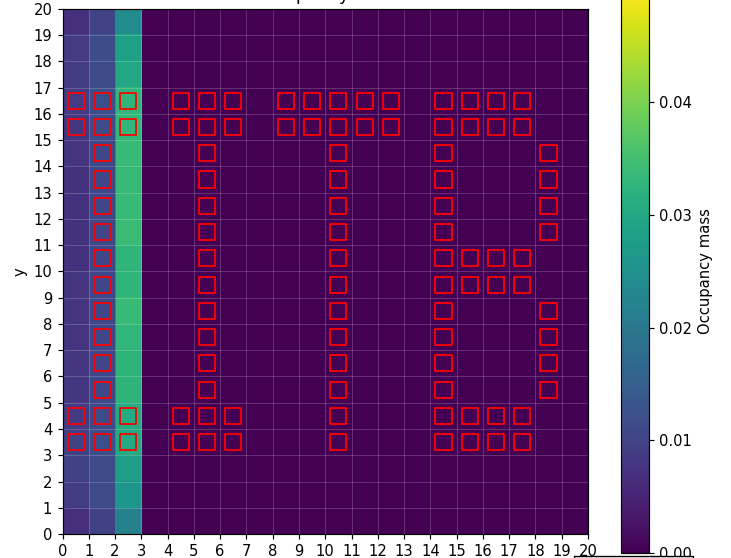
\includegraphics[width=0.95\linewidth]{example_start.png}
}{
    \fbox{\parbox[c][2.8cm][c]{0.92\linewidth}{\centering Start stage image}}
}
\\[-0.2em]\scriptsize Start
\end{minipage}
\hfill
\begin{minipage}{0.28\textwidth}
\centering
\IfFileExists{example_mid.png}{
    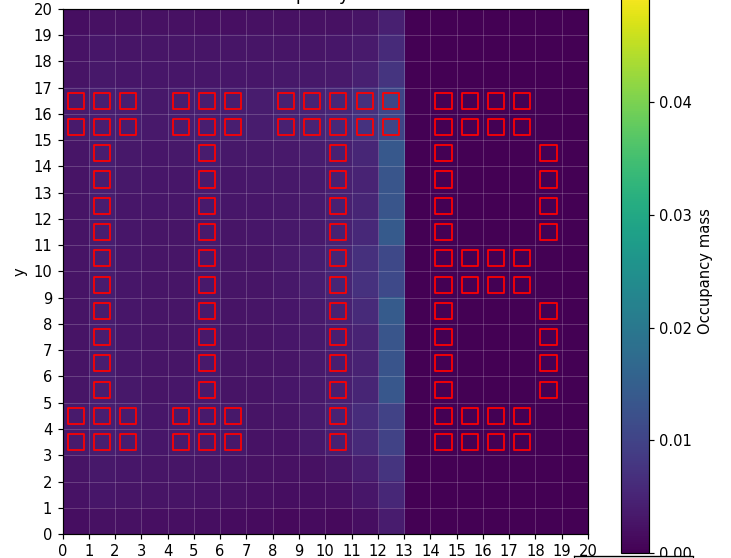
\includegraphics[width=0.95\linewidth]{example_mid.png}
}{
    \fbox{\parbox[c][2.8cm][c]{0.92\linewidth}{\centering Mid stage image}}
}
\\[-0.2em]\scriptsize Mid
\end{minipage}
\hfill
\begin{minipage}{0.28\textwidth}
\centering
\IfFileExists{example_end.png}{
    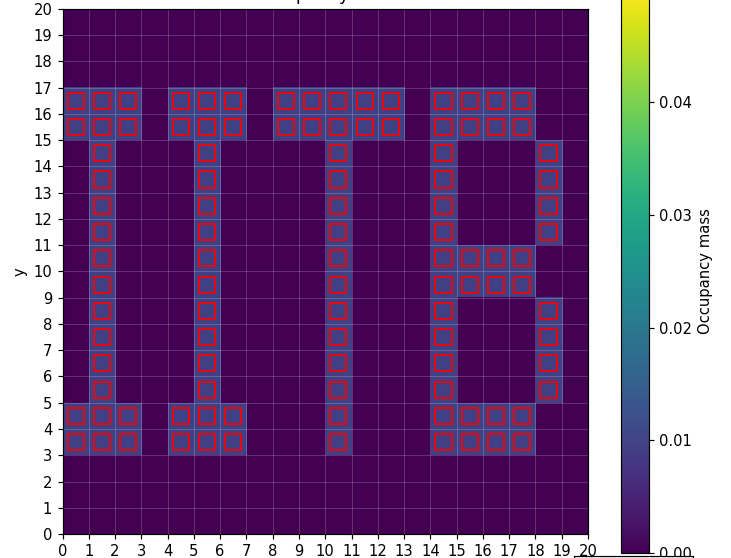
\includegraphics[width=0.95\linewidth]{example_end.png}
}{
    \fbox{\parbox[c][2.8cm][c]{0.92\linewidth}{\centering End stage image}}
}
\\[-0.2em]\scriptsize End
\end{minipage}
\caption{IITB destination example at start, intermediate, and end stages of policy rollout.}
\label{fig:iitb-multistage}
\end{figure}

\end{example}

\begin{example}[Warehouse Navigation with Path Concentration]\label{ex:concentration}
Consider a $2 \times 5$ warehouse grid. Robots must transport items from start to destination, but the warehouse monitoring system can only effectively track robots when they move in concentrated groups rather than being dispersed across multiple paths.

Define two route corridors:
\begin{itemize}
    \item $R_1 = \{s_{0,0}, s_{1,0}, s_{2,0}, s_{3,0}, s_{4,0}\}$ (bottom row)
    \item $R_2 = \{s_{0,1}, s_{1,1}, s_{2,1}, s_{3,1}, s_{4,1}\}$ (top row)
\end{itemize}

\textbf{Objective:} Transport all robots to destination while keeping them concentrated in a single corridor for effective monitoring.

\textbf{Why Distributional Rewards:} An individual robot cannot determine whether the swarm is concentrated or dispersed—this requires knowing the global distribution $\mu$.

\textbf{Reward Formulation:} For each corridor $R_i$, let $\phi_i(\mu) = \sum_{s \in R_i} \mu(s)$ be the fraction of robots in that corridor. Define:
\[
R_{\text{dist}}(\mu) = -c \cdot \sum_{s \notin S_{\text{dest}}} \mu(s) + \max_{i \in \{1,2\}} (-\lambda \cdot \phi_i(\mu))
\]
where $S_{\text{dest}} = \{s_{4,0}, s_{4,1}\}$ are destination cells and $c, \lambda > 0$.

The first term penalizes robots not yet at destination (encouraging speed). The max-linear term penalizes the *less occupied* corridor: when robots split evenly with $\phi_1 = \phi_2 = 0.5$, we get $\max(-0.5\lambda, -0.5\lambda) = -0.5\lambda$. When concentrated with $\phi_1 = 0.9, \phi_2 = 0.1$, we get $\max(-0.9\lambda, -0.1\lambda) = -0.1\lambda$ (less penalty). An optimal policy concentrates robots in one corridor while minimizing travel time.
\end{example}

\begin{example}{ (Reach Avoidance)} \label{ex:Reach-avoid}
We can also represent the safety constraints as mentioned in 
\cite{akshay2024certifiedpolicyverificationsynthesis} as soft constraints 
(by adding huge negative penalty) using distributional rewards.

Say we are given an MDP planning problem with given safety constraints of the form 
($\sum_{s}\mu(s)\cdot c_s^{i} \geq d^{i}$ for $i \in [1,N_c]$), then we can represent a reward function as

\[
\begin{aligned}
R_{\text{dist}}(\mu)
&= -c \cdot \sum_{s \notin S_{\text{dest}}} \mu(s) \\
&\quad + \sum_{i \in N_c} P_i \cdot \min\!\left(0, \sum_{s} \mu(s)\cdot c_s^{i} - d^{i}\right)
\end{aligned}
\]
\end{example}



\begin{example}[Formation with Obstacle Avoidance]\label{ex:army-formation}
An army advances across a $10\times6$ grid from left to right.
Two competing objectives drive the reward:
\emph{formation cohesion} (keep units concentrated in a tight block) and
\emph{danger avoidance} (stay away from hazardous regions).
Both depend on the \emph{global} distribution~$\mu$ and cannot be
expressed as state-based rewards.


\begin{figure}[h]
\centering
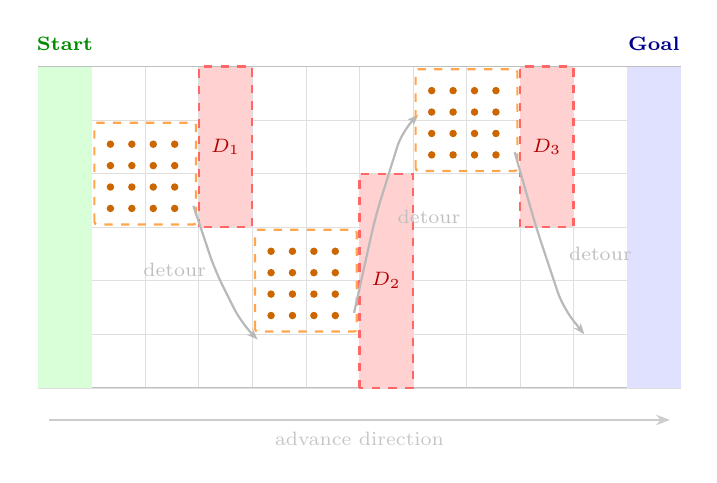
\begin{tikzpicture}[scale=0.68]
  % Grid
  \draw[step=1cm, gray!25, very thin] (0,0) grid (12,6);
  \draw[gray!50, thin] (0,0) rectangle (12,6);

  % Start / Goal columns
  \fill[green!15] (0,0) rectangle (1,6);
  \fill[blue!12]  (11,0) rectangle (12,6);
  \node[above, font=\scriptsize\bfseries, green!55!black] at (0.5,6.12) {Start};
  \node[above, font=\scriptsize\bfseries, blue!55!black]  at (11.5,6.12) {Goal};

  % Danger zone D1: cols 3–4, rows 3–6 (blocks upper half)
  \fill[red!18] (3,3) rectangle (4,6);
  \draw[red!60, thick, dashed] (3,3) rectangle (4,6);
  \node[font=\scriptsize, red!70!black] at (3.5,4.5) {$D_1$};

  % Danger zone D2: cols 6–7, rows 0–4 (blocks lower two-thirds)
  \fill[red!18] (6,0) rectangle (7,4);
  \draw[red!60, thick, dashed] (6,0) rectangle (7,4);
  \node[font=\scriptsize, red!70!black] at (6.5,2) {$D_2$};

  % Danger zone D3: cols 9–10, rows 3–6 (blocks upper half)
  \fill[red!18] (9,3) rectangle (10,6);
  \draw[red!60, thick, dashed] (9,3) rectangle (10,6);
  \node[font=\scriptsize, red!70!black] at (9.5,4.5) {$D_3$};

  % === (i) Form: cols 1–2, rows 3–4 (upper area, before D1) ===
  \draw[orange!70, thick, dashed, rounded corners=1pt]
       (1.05,3.05) rectangle (2.95,4.95);
  \foreach \x in {1.35,1.75,2.15,2.55}{
    \foreach \y in {3.35,3.75,4.15,4.55}{
      \fill[orange!80!black] (\x,\y) circle (0.07cm);
    }}
  \node[below, font=\scriptsize\bfseries, orange!70!black]
       at (2,2.85) {};

  % Detour south around D1: army at rows 3–4, D1 blocks rows 3–6
  \draw[-{Stealth[length=4pt]}, gray!55, thick, rounded corners=6pt]
       (2.9,3.4) -- (3.3,2.2) -- (3.8,1.2) -- (4.1,0.9);
  \node[font=\scriptsize, gray!50] at (2.55,2.2) {detour};

  % === (iii) Reform: cols 4–5, rows 0–1 (bottom, between D1 and D2) ===
  \draw[orange!70, thick, dashed, rounded corners=1pt]
       (4.05,1.05) rectangle (5.95,2.95);
  \foreach \x in {4.35,4.75,5.15,5.55}{
    \foreach \y in {1.35,1.75,2.15,2.55}{
      \fill[orange!80!black] (\x,\y) circle (0.07cm);
    }}
  \node[above, font=\scriptsize\bfseries, orange!70!black]
       at (5,3.15) {};

  % Detour north around D2: army at rows 0–1, D2 blocks rows 0–4
  \draw[-{Stealth[length=4pt]}, gray!55, thick, rounded corners=6pt]
       (5.9,1.4) -- (6.3,3.2) -- (6.8,4.8) -- (7.1,5.1);
  \node[font=\scriptsize, gray!50] at (7.3,3.2) {detour};

  % === (v) Reform: cols 7–8, rows 4–5 (top, between D2 and D3) ===
  \draw[orange!70, thick, dashed, rounded corners=1pt]
       (7.05,4.05) rectangle (8.95,5.95);
  \foreach \x in {7.35,7.75,8.15,8.55}{
    \foreach \y in {4.35,4.75,5.15,5.55}{
      \fill[orange!80!black] (\x,\y) circle (0.07cm);
    }}
  \node[below, font=\scriptsize\bfseries, orange!70!black]
       at (8,3.85) {};

  % Detour south around D3: army at rows 4–5, D3 blocks rows 3–6
  \draw[-{Stealth[length=4pt]}, gray!55, thick, rounded corners=6pt]
       (8.9,4.4) -- (9.3,3.0) -- (9.8,1.5) -- (10.2,1.0);
  \node[font=\scriptsize, gray!50] at (10.5,2.5) {detour};

  % Advance arrow
  \draw[-{Stealth[length=5pt]}, gray!40, thick]
       (0.2,-0.6) -- (11.8,-0.6);
  \node[below, font=\scriptsize, gray!45] at (6,-0.65) {advance direction};
\end{tikzpicture}

\caption{Army advances through a $12\!\times\!6$ grid with three staggered
danger zones that force alternating detours.
}
\label{fig:army-formation}
\end{figure}


\paragraph{Setup.}
Let $S=\{(i,j): i\in\{1,\ldots,10\},\,j\in\{1,\ldots,6\}\}$ be the
60-cell state space, with $\mu\in\Delta(S)$ the distribution of soldiers.
For any subset $U\subseteq S$, write
$\phi_U(\mu)=\sum_{s\in U}\mu(s)$ for the total mass in~$U$.

\paragraph{Reward function.}
Fix a window size $r=3$. Let $\mathcal{W}$ be the family of all
$r\!\times\!r$ sliding windows:
\[
  \mathcal{W}
  = \bigl\{
      W_{ij} = \{(i',j') : i \le i' < i{+}3,\; j \le j' < j{+}3\}
    \bigr\},
\]
so $|\mathcal{W}| = 8\times4 = 32$ windows in total.
Let $D_1,D_2,D_3\subset S$ be the three danger zones shown above,
each with a safe-mass threshold $\kappa_\ell\in(0,1)$.
The reward is:
\begin{equation}\label{eq:army-reward}
  R_{\mathrm{dist}}(\mu)
  \;=\;
  \underbrace{\alpha\,\mathbf{r}_{\mathrm{prog}}^{\!\top}\mu\vphantom{\sum}}_{\text{progress}}
  \;+\;
  \underbrace{\beta \max_{W\in\mathcal{W}}\mathbf{1}_{W}^{\!\top}\mu}_{\text{formation}}
  \;-\;
  \underbrace{\sum_{\ell=1}^{3}C_\ell
    \max\!\bigl(0,\,\phi_{D_\ell}(\mu)-\kappa_\ell\bigr)}_{\text{danger penalty}},
\end{equation}
where $\alpha,\beta,C_\ell>0$ are tunable weights and each term captures
a distinct aspect of the objective:

\begin{itemize}
\item \textbf{Progress} $(\alpha\,\mathbf{r}_{\mathrm{prog}}^{\!\top}\mu)$:
  The vector $\mathbf{r}_{\mathrm{prog}}\in\mathbb{R}^{|S|}$ assigns
  $\mathbf{r}_{\mathrm{prog}}(i,j)=i/10$ to each cell, so this term
  rewards mass that has advanced further to the right.
  It equals the (normalised) average column index of the army.

\item \textbf{Formation}
  $(\beta\max_{W\in\mathcal{W}}\mathbf{1}_{W}^{\!\top}\mu)$:
  $\mathbf{1}_W\in\{0,1\}^{|S|}$ is the indicator of window~$W$, so
  $\mathbf{1}_W^{\!\top}\mu = \phi_W(\mu)$ is the fraction of the army
  inside~$W$. Maximising over all windows finds the tightest
  $3\!\times\!3$ block containing the most mass.
  This term equals~$1$ when the army is fully concentrated in some
  window and is small when dispersed.

\item \textbf{Danger penalty}
  $(\sum_\ell C_\ell\max(0,\phi_{D_\ell}(\mu)-\kappa_\ell))$:
  If the mass inside danger zone $D_\ell$ exceeds threshold
  $\kappa_\ell$, a penalty proportional to the excess is incurred.
  This forces the army to route around hazardous regions.
\end{itemize}



\end{example}




% I think the other swarm formation example should be improved , so I will add it later


\section{Optimality of Memoryless Distributional Policies}\label{sec:analysis} 

Before solving for optimal strategy for finding expected reward , we would like to know first what type of strategies are sufficient and what are not.

In this Section we show 2 results 
\begin{enumerate}
    \item State-based memoryless policies are insufficient for optimizing expected reward over infinte horizon .
    \item Distributional based memoryless policies are sufficient for optimizing expected reward over infinite horizon
\end{enumerate}



\begin{theorem}\label{thm:markov-insufficient} 
State-based memoryless policies are not sufficient for optimizing expected reward under distributional reward functions.
\end{theorem} 

\begin{proof}  
Consider states $S = \{s_1, s_2, s_3\}$, actions $A = \{a_1, a_2\}$, with transitions shown in Figure~\ref{fig:counterexample}.

\begin{figure}[h]
\centering
\begin{tikzpicture}[
    state/.style={circle, draw, thick, minimum size=0.9cm, font=\small},
    every edge/.style={draw, ->, >=Stealth, thick},
    node distance=2.5cm
]
    \node[state] (s1) {$s_1$};
    \node[state, right=of s1] (s2) {$s_2$};
    \node[state, below=1.8cm of $(s1)!0.5!(s2)$] (s3) {$s_3$};
    
    \path (s1) edge[loop above, looseness=5] node[above, font=\scriptsize] {$a_1\!:\!0.5$} (s1);
    \path (s1) edge[bend left=15] node[above, font=\scriptsize] {$a_1\!:\!0.5$} (s2);
    \path (s1) edge node[left, font=\scriptsize] {$a_2\!:\!1$} (s3);
    \path (s2) edge[loop above, looseness=5] node[above, font=\scriptsize] {$a_1\!:\!1$} (s2);
    \path (s2) edge node[right, font=\scriptsize] {$a_2\!:\!1$} (s3);
    \path (s3) edge[loop below, looseness=5] node[below, font=\scriptsize] {$a_1,a_2\!:\!1$} (s3);
\end{tikzpicture}
\caption{Counterexample MDP showing insufficiency of state-based policies.}
\label{fig:counterexample}
\end{figure}

Define $R_{\text{dist}}(\mu, \pi) = 1$ if $\mu = (0.5, 0.5,0)$  and $\pi_{s1}(a2) = 1 $, otherwise $0$. With initial distribution $\mu_0 = (1, 0, 0)$:

\textbf{Distributional strategy achieving positive reward:} At $t=0$: play $a_1$ at $s_1$ $\Rightarrow$ $\mu_1 = (0.5, 0.5, 0)$. At $t=1$: play $a_2$ at both $s_1$ and $s_2$ $\Rightarrow$ $\mu_2 = (0, 0, 1)$  . This yields expected reward $\gamma  > 0$.

\textbf{No state based memoryless policy achieves positive reward:} To earn reward requires (1) reaching $\mu = (0.5, 0.5, 0)$ by playing $a_1$ at $s_1$, and (2)  playing $a_2$ at $s_1$. But a state based memoryless policy uses the \emph{same} action at $s_1$ at all times—it cannot play $a_1$ first then switch to $a_2$.
\end{proof}

\begin{theorem}\label{thm:memoryless-sufficient}
Memoryless distributional policies are sufficient for optimizing expected reward over infinite horizon under distributional reward functions.
\end{theorem}

\begin{proof}
Let $\pi^*$ be an optimal policy (possibly history-dependent) generating trajectory $\tau = (\mu_0, \mu_1, \mu_2, \ldots)$.

\textbf{Case 1: All distributions in $\tau$ are distinct.} Define $\tilde{\pi}(\mu_t)$ to be the action distribution that $\pi^*$ selects at time $t$. Since each $\mu_t$ appears exactly once, $\tilde{\pi}$ is well-defined and achieves identical expected reward.

\textbf{Case 2: Some distribution repeats.} Suppose $\mu$ appears at times $t_1 < t_2$.

\begin{claim}
If an optimal policy visits $\mu$ at two different times, there exists an optimal policy cycling through $\mu$ infinitely with identical intermediate trajectories.
\end{claim}

Let $R_{\text{cycle}} = \sum_{t=t_1}^{t_2-1} \gamma^{t-t_1} r_t$. Since $\pi^*$ is optimal and returns to $\mu$:
\[
V^*(\mu) = R_{\text{cycle}} + \gamma^{t_2-t_1} \cdot V^*(\mu),
\]
showing repeated cycles achieve optimal value.

From this claim, there exists an optimal policy whose trajectory is eventually periodic. Define $\tilde{\pi}(\nu)$ as the action distribution selected at distribution $\nu$. This is well-defined since (a) before the cycle, each distribution appears at most once, and (b) within the cycle, we have a unique action for each distribution. This memoryless policy $\tilde{\pi}$ achieves optimal expected reward.
\end{proof}




\section{Hardness Results -- New section }
\label{sec:hardness-results}

\begin{theorem}[Policy evaluation is Skolem hard]
\label{thm:policy_evalution_hardness}


Given an MDP, a distributional reward function, and a  policy $\pi$, deciding whether the expected total discounted reward over an infinite horizon is greater than $0$ is Skolem-hard.

\end{theorem}

\begin{proof}
We prove the result via reduction from a known Skolem-hard problem.

Given a Markov chain $(S,T)$, an initial state $s_{start}$, a state $s^\star \in S$, and a threshold $c \in (0,1)$, decide whether
\[
\exists t \ge 0 \text{ such that } \mu_t(s^\star) > c.
\]

is Skolem-hard.

Given such a Markov chain, we construct an equivalent MDP by assigning a single action at every state. Thus, the MDP admits exactly one policy, and its dynamics coincide with the original Markov chain.

Now define a distributional reward function:
\[
R_{\mathrm{dist}}(\mu_t) = \max\big(0, \mu_t(s_i) - c\big).
\]

Consider the total discounted reward:
\[
\sum_{t=0}^{\infty} \gamma^t R_{\mathrm{dist}}(\mu_t).
\]

Observe:
\begin{itemize}
    \item If there exists $t$ such that $\mu_t(s_i) > c$, then $R_{\mathrm{dist}}(\mu_t) > 0$ for that $t$, and hence the total reward is strictly positive.
    \item If for all $t$, $\mu_t(s_i) \le c$, then $R_{\mathrm{dist}}(\mu_t) = 0$ for all $t$, and the total reward is $0$.
\end{itemize}

Therefore, deciding whether the total reward is greater than $0$ is equivalent to deciding whether there exists $t$ such that $\mu_t(s_i) > c$.

Since the latter problem is Skolem-hard, the result follows.
\end{proof}


\begin{theorem}[Optimality Checking is Skolem-hard] \label{thm: optimality_checking_hardness}

Let $\mathcal{M} = (S,A,T,\gamma)$ be a finite MDP, 
$R_{\mathrm{dist}} : \Delta(S) \times \Delta(A)^{|S|} \to \mathbb{R}$ a distributional reward function, and $\pi$ is a distributional policy .

Deciding whether $\pi$ is optimal, i.e.,
\[
V^\pi(\mu_0) = \sup_{\pi'} V^{\pi'}(\mu_0),
\]
is Skolem-hard.
\end{theorem}

\begin{proof}
We reduce from the following Skolem-hard problem:

\medskip
\noindent
\textbf{Problem.} Given a Markov chain $(S,T)$, an initial state $s_{start}$, a state $s^\star \in S$, and a threshold $c \in (0,1)$, decide whether
\[
\exists t \ge 0 \text{ such that } \mu_t(s^\star) > c.
\]

\medskip

\textbf{Construction.}
From the given Markov chain, construct an MDP $\mathcal{M}'$ as follows:

\begin{itemize}
    \item State space: $S' = S \cup \{s_0, s_{\mathrm{sink}}\}$.
    
    \item Actions:
    \[
    A(s_0) = \{a_0, a_1\}, \quad
    A(s) = \{a_0\} \ \forall s \in S, \quad
    A(s_{\mathrm{sink}}) = \{a_0\}.
    \]
    
    \item Transitions:
    \begin{itemize}
        \item From $s_0$:
        \begin{itemize}
            \item $a_0$: transitions to  $s_{start}$ of markov chain 
            \item $a_1$: transitions to $s_{\mathrm{sink}}$
        \end{itemize}
        \item For $s \in S$: follow the original Markov chain dynamics $T$
        \item $s_{\mathrm{sink}}$ is absorbing
    \end{itemize}
\end{itemize}

\medskip

\textbf{Reward function.}
Define the distributional reward:
\[
R_{\mathrm{dist}}(\mu) = \max\big(0, \mu(s^\star) - c \big).
\]

\medskip

\textbf{Policies.}
Consider the policy $\pi$ defined by:
\[
\pi(s_0) = a_1, \quad \pi(s) = a_0 \ \forall s \neq s_0.
\]
This policy immediately transitions to the sink state and hence yields zero reward:
\[
V^\pi(\mu_0) = 0.
\]

Consider an alternative policy $\pi'$:
\[
\pi'(s_0) = a_0, \quad \pi'(s) = a_0 \ \forall s \in S.
\]
This policy simulates the original Markov chain.

\medskip

\textbf{Correctness of reduction.}

\begin{itemize}
    \item If $\exists t$ such that $\mu_t(s^\star) > c$, then
    \[
    R_{\mathrm{dist}}(\mu_t) > 0,
    \]
    and hence $V^{\pi'}(\mu_0) > 0$. Therefore $\pi$ is \emph{not} optimal.
    
    \item If for all $t$, $\mu_t(s^\star) \le c$, then
    \[
    R_{\mathrm{dist}}(\mu_t) = 0 \quad \forall t,
    \]
    implying $V^{\pi''}(\mu_0) = 0 \quad \forall \pi''$. Hence $\pi$ is optimal.
\end{itemize}

\medskip

Thus, deciding whether $\pi$ is optimal is equivalent to deciding whether
\[
\exists t \text{ such that } \mu_t(s^\star) > c,
\]
which is Skolem-hard.

\medskip

Therefore, optimality checking is Skolem-hard.
\end{proof}


\begin{theorem}[Optimal policy synthesis is skolem hard]\label{thm: optimal_synthesis_hardness}
Given an MDP with a distributional reward function, computing an optimal policy for the infinite-horizon discounted objective is Skolem-hard.
\end{theorem}

\begin{proof}
We reduce from the following Skolem-hard problem: given a Markov chain $(S,T)$, an initial state $s_{start}$, a state $s_i \in S$, and a threshold $c \in (0,1)$, decide whether
\[
\exists t \ge 0 \text{ such that } \mu_t(s_i) > c.
\]

\medskip
\noindent
\textbf{Construction.}
From the given Markov chain, construct an MDP $\mathcal{M}'$ as follows.
The state space is
\[
S' = S \cup \{s_0\}.
\]
The action set is
\[
A = \{a_0,a_1\}.
\]
The available actions are:
\[
A(s_0)=\{a_0\}, \qquad A(s)=\{a_0,a_1\}\ \text{for all } s\in S.
\]
The transitions are defined by:
\begin{itemize}
    \item from $s_0$, action $a_0$ moves to the initial state $\s_{start}$ of the markov chain ;
    \item for every $s\in S$, action $a_0$ follows the original Markov chain transition matrix $T$;
    \item for every $s\in S$, action $a_1$ sends the entire mass to $s_0$.
\end{itemize}

\medskip
\noindent
\textbf{Reward function.}
Define the distributional reward at time $t$ by
\[
R_{\mathrm{dist}}(\mu_t)
=
-\mu_t(s_0)
-
M\cdot \max(\mu_t(s_i)-c,0),
\]
% where
% \[
% M=\frac{1000}{\gamma}.
% \]
The total objective is the infinite-horizon discounted return
\[
\sum_{t=0}^{\infty}\gamma^t R_{\mathrm{dist}}(\mu_t).
\]

\medskip
\noindent
\textbf{Correctness of the reduction.}
Let $\pi^0$ denote the policy that always selects $a_0$ whenever $a_1$ is not chosen. Since $a_0$ is the only action at $s_0$, this means that $\pi^0$ follows the original Markov chain and never uses $a_1$.

Suppose that, under this trajectory, there exists a first time $N$ such that
\[
\mu_N(s_i)>c.
\]
Then the policy $\pi^0$ incurs a penalty of at least
\[
-M\gamma^N
\]
from the term $-M\cdot \max(\mu_t(s_i)-c,0)$, and the additional contribution from the term
$-\mu_t(s_0)$ is nonpositive. Hence
\[
V^{\pi^0}(\mu_0)\le -M\gamma^N.
\]

Now consider an alternative policy $\pi^1$ that uses $a_1$ at time $N-1$ and thereafter continues in the same manner whenever needed so as to prevent the distribution from reaching the threshold state $s_i$ at time $N$.
Under this policy, the penalty term $-M\cdot \max(\mu_t(s_i)-c,0)$ is avoided at time $N$, and the only unavoidable cost is the term $-\mu_t(s_0)$.
Since $\mu_t(s_0)\le 1$ for every $t$, we obtain the lower bound
\[
V^{\pi^1}(\mu_0)
\ge
-\sum_{t=N}^{\infty}\gamma^t
=
-\frac{\gamma^{N}}{1-\gamma}.
\]

take
\[
M > \frac{1}{(1-\gamma)},
\]
we have
\[
-\frac{\gamma^{N}}{1-\gamma} > -M\gamma^N.
\]
Therefore,
\[
V^{\pi^1}(\mu_0) > V^{\pi^0}(\mu_0),
\]
so the policy that uses only $a_0$ is not optimal , the optimal must take action $a_1$ at some point .

On the other hand, if
\[
\mu_t(s_i)\le c \quad \text{for all } t,
\]
then the penalty term is never activated. In that case, any use of $a_1$ only introduces extra visits to $s_0$, and hence extra cost through the term $-\mu_t(s_0)$. Therefore, an optimal policy never uses $a_1$.

Thus, an optimal policy uses $a_1$ if and only if the threshold event
\[
\exists t \ge 0 \text{ such that } \mu_t(s_i)>c
\]
occurs in the original Markov chain. Hence computing an optimal policy allows us to decide a Skolem-hard problem.

Therefore, optimal policy synthesis for this distributional-reward MDP is Skolem-hard.
\end{proof}

\begin{remark}[Intuition]
If the threshold is reached at time $N$, then the policy that never uses $a_1$ pays the large penalty $-M\gamma^N$.
A policy that switches to $a_1$ before that point avoids this penalty and pays at most
\[
-\frac{\gamma^{N}}{1-\gamma},
\]
which is strictly larger. This is exactly why the all-$a_0$ policy cannot be optimal when the threshold is reachable.
\end{remark}


\paragraph{Conclusion.}
In the infinite-horizon setting, all problems involving distributional reward functions—namely policy evaluation, optimality verification, and optimal policy synthesis—are Skolem-hard.


Given that solving for infinite horizon is a hard problem even for simple reward functions as shown in \ref{thm:policy_evalution_hardness} ,\ref{thm: optimality_checking_hardness}, \ref{thm: optimal_synthesis_hardness} lets first try to solve the problem for finite horizon case 


\section{Convex Optimization Solution for concave reward functions in Finite-Horizon setting }
\label{sec:convex-finite-horizon}

For the finite horizon setting , if the distributional reward function is concave , the reward optimization problem can be written as convex optimization problem ( maximizing over concave function ) 

\begin{definition}[Occupancy Measure]
For each time step $t \in \{0,\dots,T-1\}$, define
\[
x_t(s,a) := \mu_t(s)\,\pi_t(a\mid s), \qquad s \in S,\ a \in A.
\]
Then $\mu_t(s) = \sum_{a \in A} x_t(s,a)$ for every $s \in S$.
\end{definition}

Using these variables, the distributional dynamics become linear:
\[
\begin{aligned}
    \mu_{t+1}(s') = \sum_{s \in S}\sum_{a \in A} x_t(s,a)\,T(s,a,s'), \\
    \quad \forall s' \in S,\ \forall t \in \{0,\dots,T-1\}.
\end{aligned}
\]

We now formulate the finite-horizon problem directly in terms of $\{x_t,\mu_t\}$:
\[
\begin{aligned}
\max_{\{\mu_t,x_t\}} \quad &
\sum_{t=0}^{T-1} \gamma^t R_{\mathrm{dist}}(\mu_t,x_t) \\
\text{s.t.}\quad
& \mu_0 = \mu_{\mathrm{init}}, \\
& \sum_{a \in A} x_t(s,a) = \mu_t(s), \qquad \forall s \in S,\ \forall t, \\
& \mu_{t+1}(s') = \sum_{s \in S}\sum_{a \in A} x_t(s,a)\,T(s,a,s'),  \forall s' \in S,\ \forall t, \\
& x_t(s,a) \ge 0, \qquad \forall s \in S,\ a \in A,\ \forall t.
\end{aligned}
\]

 If the reward is affine in the occupancies, the problem reduces to a linear program.


 

\begin{remark}[Policy Recovery]
Given an optimal feasible solution $\{x_t^\star,\mu_t^\star\}$, an optimal policy is recovered by
\[
\pi_t^\star(a\mid s)=
\begin{cases}
\dfrac{x_t^\star(s,a)}{\mu_t^\star(s)}, & \mu_t^\star(s)>0,\\[1.2ex]
\text{arbitrary in }\Delta(A), & \mu_t^\star(s)=0.
\end{cases}
\]
\end{remark}


\begin{note}
    The present solution will optimize over all possible policies , which can be time varying , the \ref{thm:memoryless-sufficient} only states that memoryless policies are sufficient in infinite horizon setting not in finite horizon 
\end{note}

\begin{remark}
    The examples \ref{ex:swarm-congestion},\ref{ex:Reach-avoid} can solved using above approach for finite horizon setting , in fact for these examples can be directly formulated as an \textbf{Linear program } as piecewise-linear concave rewards of the form $-\max(0,\text{linear})$ or $\min(0,\text{linear})$ can be represented exactly using linear constraints and auxiliary variables
\end{remark}




\paragraph{Slack Variable Reformulation.}

If a term of -max(x,y) is present in the reward function , create a variable z ,
\[
\begin{aligned}
z &\ge x, y
\end{aligned}
\] , and now replace $-\max(x,y)$ term with $-z$ .



\section{Value Iteration solution for convex reward functions }\label{sec:value-iteration}
The convex optimization approach of Section~\ref{sec:convex-finite-horizon} 
handles concave distributional reward functions. We now consider the 
complementary class: \emph{convex} reward functions. Specifically, we focus 
on rewards that are \textbf{max-linear} in the distribution:
\[
    R_{\mathrm{dist}}(\mu, \pi) 
    \;=\; \max_{i \in [K]} \,\mathbf{a}_{\pi,i}^\top \mu,
\]
where $\mathbf{a}_{\pi,i} \in \mathbb{R}^{|S|}$ are reward vectors indexed by 
the policy $\pi$ and mode $i \in [K]$. Each term $\mathbf{a}_{\pi,i}^\top \mu$ 
is linear in $\mu$, so the reward is a piecewise-linear convex function of 
$\mu$ for every fixed $\pi$.

\begin{note}
    Any convex function can be approximated arbitrarily closely by a 
    max-linear function~\citep{NIPS2010_68053af2}, so this class is broadly 
    expressive. In particular, the formation reward 
    $\beta\max_{W \in \mathcal{W}}\mathbf{1}_W^\top\mu$ from 
    Example~\ref{ex:army-formation} is directly max-linear with $K = |\mathcal{W}|$ 
    and $\mathbf{a}_i = \beta\,\mathbf{1}_{W_i}$.
\end{note}


\paragraph{Restriction to deterministic policies : } We optimize over the class of 
\emph{deterministic} distributional policies .




\begin{definition}[Deterministic Distributional Policy]
A \emph{deterministic distributional policy} at time $t$ is a mapping 
$\pi_t : \Delta(S) \to A^{S}$ that assigns to each distribution 
$\mu \in \Delta(S)$ a single action $\pi_t(\mu)(s) \in A$ at every state $s$.
\end{definition}

Let $\Pi$ denote the (finite) set of all deterministic policies. Under any 
$\pi \in \Pi$, the distribution evolves \emph{linearly}:
\[
    \mu'(s') \;=\; \sum_{s \in S} \mu(s)\,T(s,\,\pi(s),\,s') 
              \;=\; (T_\pi^\top \mu)(s'),
\]
where $[T_\pi]_{ss'} = T(s,\pi(s),s')$. This linearity is the key 
structural property that makes the value iteration algorithm tractable.

\subsection{Finite-Horizon Value Iteration}

\begin{definition}[Optimal Value Function]
For $t_0 \in \{0,\ldots,T\}$ and $\mu \in \Delta(S)$, the 
\emph{optimal value function} is:
\[
    V_{t_0}^*(\mu) 
    \;=\; \sup_{\{\pi_t\}} \;\mathbb{E}\!\left[
        \sum_{t=t_0}^{T-1} \gamma^{t-t_0} R_{\mathrm{dist}}(\mu_t, \pi_t(\mu_t))
        \,\Big|\, \mu_{t_0} = \mu
    \right],
\]
where the supremum is over all sequences of deterministic policies 
$\{\pi_t\}_{t=t_0}^{T-1}$.
\end{definition}

\begin{proposition}[Bellman Recursion]\label{prop:bellman-finite}
For all $t_0 \in \{0,\ldots,T-1\}$ and $\mu \in \Delta(S)$:
\[
    V_{t_0}^*(\mu) 
    \;=\; \max_{\pi \in \Pi} \left[ 
        R_{\mathrm{dist}}(\mu,\,\pi) \;+\; \gamma\cdot V_{t_0+1}^*(T_\pi^\top \mu)
    \right],
\]
with boundary condition $V_T^*(\mu) = 0$ for all $\mu \in \Delta(S)$.
\end{proposition}

\begin{proof}
Separating the $t = t_0$ reward term and applying the principle of 
optimality to the remaining horizon gives:

\begin{align}
V_{t_0}^*(\mu) 
&= \max_{\pi \in \Pi}\!\Bigg[
    R_{\mathrm{dist}}(\mu,\pi) \\
& + \gamma \cdot \sup_{\{\pi_t\}_{t>t_0}}
    \mathbb{E}\!\left[
        \sum_{t=t_0+1}^{T-1}\!\gamma^{t-t_0-1}
        R_{\mathrm{dist}}(\mu_t,\pi_t)
        \,\middle|\,
        \mu_{t_0+1} = T_\pi^\top\mu
    \right]
\Bigg].
\end{align}


The inner supremum equals $V_{t_0+1}^*(T_\pi^\top\mu)$ by definition.
\end{proof}

\begin{theorem}[Value Function is Max-Linear]\label{thm:finite-horizon}
For all $t \in \{0,\ldots,T\}$, the optimal value function is max-linear:
\[
    V_t^*(\mu) \;=\; \max_{\mathbf{v} \in \Gamma_t}\; \mathbf{v}^\top \mu,
\]
where $\Gamma_t \subset \mathbb{R}^{|S|}$ is a finite set of vectors.
\end{theorem}

\begin{proof}
We proceed by backward induction on $t$.

\medskip\noindent
\textbf{Base case} ($t = T$). $V_T^*(\mu) = 0 = \mathbf{0}^\top\mu$ for all $\mu$, 
so set $\Gamma_T = \{\mathbf{0}\}$.

\medskip\noindent
\textbf{Inductive step.} Suppose $V_{t+1}^*(\mu) = \max_{\mathbf{v} \in \Gamma_{t+1}} 
\mathbf{v}^\top\mu$ for some finite set $\Gamma_{t+1}$.  By the Bellman recursion 
(Proposition~\ref{prop:bellman-finite}) and the max-linear reward:
\begin{align*}
    V_t^*(\mu) 
    &= \max_{\pi \in \Pi}\left[
        \max_{i \in [K]} \mathbf{a}_{\pi,i}^\top\mu 
        \;+\; \gamma \max_{\mathbf{v} \in \Gamma_{t+1}} \mathbf{v}^\top T_\pi^\top\mu
    \right] \\
    &= \max_{\pi \in \Pi}\;
       \max_{i \in [K]}\;
       \max_{\mathbf{v} \in \Gamma_{t+1}}
       \left(\mathbf{a}_{\pi,i} + \gamma\, T_\pi\,\mathbf{v}\right)^\top\!\mu,
\end{align*}
where the second equality uses the fact that $i$ and $\mathbf{v}$ are 
independently optimized, so
$\max_i x_i + \max_j y_j = \max_{i,j}(x_i + y_j)$.

Setting
\[
    \Gamma_t 
    \;=\; \bigcup_{\pi \in \Pi}\;\bigcup_{i \in [K]}
          \Bigl\{\mathbf{a}_{\pi,i} + \gamma\,T_\pi\,\mathbf{v}
                 \;:\; \mathbf{v} \in \Gamma_{t+1}\Bigr\}
\]
gives $V_t^*(\mu) = \max_{\mathbf{w} \in \Gamma_t}\mathbf{w}^\top\mu$.
Since $|\Pi|$, $K$, and $|\Gamma_{t+1}|$ are all finite, so is $|\Gamma_t|$.
\end{proof}

Algorithm~\ref{alg:finite-horizon} implements this backward recursion directly.

\begin{algorithm}[t]
\caption{Finite-Horizon Value Iteration for Max-Linear Distributional Rewards}
\label{alg:finite-horizon}
\begin{algorithmic}[1]
\STATE \textbf{Input:} Horizon $T$, discount $\gamma$, transition matrices 
       $\{T_\pi\}_{\pi \in \Pi}$, reward vectors $\{\mathbf{a}_{\pi,i}\}_{\pi,i}$
\STATE \textbf{Initialize:} $\Gamma_T \gets \{\mathbf{0}\}$
\FOR{$t = T-1,\; T-2,\; \ldots,\; 0$}
    \STATE $\Gamma_t \gets \emptyset$
    \FOR{each policy $\pi \in \Pi$}
        \FOR{each reward mode $i \in [K]$}
            \FOR{each vector $\mathbf{v} \in \Gamma_{t+1}$}
                \STATE $\Gamma_t \gets \Gamma_t \cup 
                       \{\mathbf{a}_{\pi,i} + \gamma\, T_\pi\,\mathbf{v}\}$
            \ENDFOR
        \ENDFOR
    \ENDFOR
    \STATE \textbf{(Optional)} Remove dominated vectors from $\Gamma_t$
\ENDFOR
\STATE \textbf{Output:} $\{\Gamma_t\}_{t=0}^{T}$
\end{algorithmic}
\end{algorithm}

Given the output $\{\Gamma_t\}$, the optimal action at time $t$ from distribution 
$\mu$ is recovered by:
\[
    \pi_t^*(\mu) 
    \;=\; \operatorname*{arg\,max}_{\pi \in \Pi}\;
          \max_{i \in [K]}\;
          \max_{\mathbf{v} \in \Gamma_{t+1}}
          \left(\mathbf{a}_{\pi,i} + \gamma\, T_\pi\,\mathbf{v}\right)^\top\!\mu.
\]

\begin{remark}[Set size and pruning]
The set $\Gamma_t$ can grow as $O\bigl((|\Pi|\cdot K)^{T-t}\bigr)$ in the 
worst case. The optional pruning step removes a vector $\mathbf{w} \in \Gamma_t$ 
if there exists $\mathbf{w}' \in \Gamma_t$ with $\mathbf{w}'^\top\mu \geq 
\mathbf{w}^\top\mu$ for all $\mu \in \Delta(S)$. This does not affect 
correctness and can 
reduce the set size in practice.
\end{remark}


\begin{remark}
    Similar methodology is used in  \cite{NIPS2010_68053af2} where the authors introduce rewards on belief states in PoMDP's and use similar value iteration algorithm of PoMDP's
\end{remark}


\section{Infinite Horizon Case -- To be done  }\label{sec:infinite-horizon}

\begin{theorem}[Existence via Contraction Mapping]\label{thm:infinite-horizon}
For discount factor $\gamma < 1$, there exists a unique optimal value function $V^*: \Delta(S) \to \mathbb{R}$ satisfying:
\[
V^*(\mu) = \max_{\pi \in \Pi} \left[ A_{\pi}^\top \mu + \gamma \cdot V^*(T_{\pi}^\top \mu) \right].
\]
\end{theorem}

\begin{proof}
Let $\mathcal{B}(\Delta(S))$ be bounded continuous functions on $\Delta(S)$ with supremum norm $\|V\|_\infty = \sup_{\mu} |V(\mu)|$—a complete metric space.

Define Bellman operator $\mathcal{T}: \mathcal{B}(\Delta(S)) \to \mathcal{B}(\Delta(S))$:
\[
(\mathcal{T}V)(\mu) = \max_{\pi \in \Pi} \left[ A_{\pi}^\top \mu + \gamma \cdot V(T_{\pi}^\top \mu) \right].
\]


\textbf{Contraction property:} For any $V_1, V_2$ and $\mu$:
\begin{align*}
|(\mathcal{T}V_1)(\mu) - (\mathcal{T}V_2)(\mu)| &\leq \max_{\pi} \gamma |V_1(T_{\pi}^\top \mu) - V_2(T_{\pi}^\top \mu)| \leq \gamma \|V_1 - V_2\|_\infty
\end{align*}
Thus $\|\mathcal{T}V_1 - \mathcal{T}V_2\|_\infty \leq \gamma \|V_1 - V_2\|_\infty$. By the Banach Fixed Point Theorem, a unique $V^* = \mathcal{T}V^*$ exists.
\end{proof}

\textbf{In the following section we reverse the time direction in value iteration algorithm }

\begin{theorem}[Convergence of Value Iteration]\label{thm:convergence}
Starting from any $V_0 \in \mathcal{B}(\Delta(S))$, the sequence $V_{k+1} = \mathcal{T}V_k$ converges uniformly:
\[
\|V_k - V^*\|_\infty \leq \gamma^k \|V_0 - V^*\|_\infty \to 0.
\]
\end{theorem}

\begin{proof}
Since $\mathcal{T}$ is a contraction with modulus $\gamma$: $\|V_{k+1} - V^*\|_\infty = \|\mathcal{T}V_k - \mathcal{T}V^*\|_\infty \leq \gamma \|V_k - V^*\|_\infty$. By induction, $\|V_k - V^*\|_\infty \leq \gamma^k \|V_0 - V^*\|_\infty$, giving geometric convergence.
\end{proof}

\textbf{Algorithm for Infinite Horizon.} The algorithm for the infinite horizon case follows the same structure as the finite horizon case but iterates until convergence. Starting with $\Gamma_0 = \{\mathbf{0}\}$, we repeatedly compute:
\[
\Gamma_{k+1} = \bigcup_{\pi \in \Pi} \{ A_{\pi} + \gamma \cdot T_{\pi} \gamma_k : \gamma_k \in \Gamma_k \}
\]
and prune dominated vectors. The iteration continues until $\|V_{k+1} - V_k\|_\infty < \epsilon$ for some convergence threshold $\epsilon > 0$, where $V_k(\mu) = \max_{\gamma \in \Gamma_k} \gamma^\top \mu$. By standard arguments using the contraction property, if $\|V_{k+1} - V_k\|_\infty < \epsilon$, then $\|V_{k+1} - V^*\|_\infty \leq \frac{\gamma \epsilon}{1 - \gamma}$. Theorem~\ref{thm:convergence} guarantees geometric convergence of this procedure.


\subsection{Computing the Supremum Norm}\label{sec:supremum-computation}

To implement value iteration, we need to compute the stopping criterion $\|V_{k+1} - V_k\|_\infty = \sup_{\mu \in \Delta(S)} |V_{k+1}(\mu) - V_k(\mu)|$. Since $V_k(\mu) = \max_{\gamma \in \Gamma_k} \gamma^\top \mu$ is piecewise linear and convex, this supremum is attained at a vertex of $\Delta(S)$.

\begin{lemma}[Supremum Computation]\label{lem:supremum}
For piecewise linear value functions $V_k(\mu) = \max_{\gamma \in \Gamma_k} \gamma^\top \mu$, the supremum norm can be computed as:
\[
\|V_{k+1} - V_k\|_\infty = \max_{s \in S} |V_{k+1}(e_s) - V_k(e_s)|
\]
where $e_s \in \Delta(S)$ is the point mass at state $s$ (i.e., $e_s(s) = 1$ and $e_s(s') = 0$ for $s' \neq s$).
\end{lemma}

\begin{proof}
Since $V_k$ is the maximum of linear functions, it is convex and piecewise linear. For convex functions over the simplex $\Delta(S)$, the maximum is attained at a vertex. The vertices of $\Delta(S)$ are precisely the point masses $\{e_s : s \in S\}$. Therefore:
\begin{align*}
\|V_{k+1} - V_k\|_\infty &= \sup_{\mu \in \Delta(S)} |V_{k+1}(\mu) - V_k(\mu)| \\
&= \max_{s \in S} |V_{k+1}(e_s) - V_k(e_s)| \\
&= \max_{s \in S} \left|\max_{\gamma \in \Gamma_{k+1}} \gamma(s) - \max_{\gamma \in \Gamma_k} \gamma(s)\right|
\end{align*}
This can be computed in $O(|S| \cdot (|\Gamma_k| +|\Gamma_{k+1}|)$ time.
\end{proof}




% To be updated based on changes made to finite horizon 


% \ak{how does the algo change.}

% \ak{need a clear section why you can lift this to randomized policies }$\to$ \bk{ I am still working on how to lift to randomized policies}


\section{Experiments : }

For concave reward function case in \ref{sec:convex-finite-horizon}:

\begin{table}[h]
\centering
\caption{Experiment runtime summary.}
\label{tab:experiment-runtime-summary}
\begin{tabular}{cccc}
\toprule
Shape & Grid Size & Is Randomized & Time Taken (s) \\
\midrule
iitb   & 20x20 & No  & 30.513 \\
smiley & 20x20 & No  & 29.260 \\
iitb   & 40x40 & No  & 350.202 \\
smiley & 40x40 & No  & 353.572 \\
iitb   & 20x20 & Yes & 201.793 \\
iitb   & 20x20 & Yes & 1000.142 (timeout) \\
smiley & 20x20 & Yes & 1000.167 (timeout) \\
smiley & 20x20 & Yes & 1000.174 (timeout) \\
iitb   & 40x40 & Yes & 1000.295 (timeout) \\
iitb   & 40x40 & Yes & 1000.211 (timeout) \\
smiley & 40x40 & Yes & 1000.248 (timeout) \\
smiley & 40x40 & Yes & 1000.301 (timeout) \\
\bottomrule
\end{tabular}
\end{table}





% \section{Conclusion}

% We introduced distributional reward functions for multi-agent MDPs, enabling optimization of collective objectives like congestion and formation quality. We provided  value iteration algorithms for finding optimal deterministic policy in both finite and infinite horizon setting with provable convergence guarantees.

% % \ak{separate these two throughout.} -> means ?

% Future work includes extending to stochastic distributional policies, developing approximation algorithms for large state spaces, and applications to real-world multi-agent systems.

% % \ak{do you have an idea of approx algos to try?} \bk {$\to$ Have some from PoMDP's , trying them}
 


% \bibliographystyle{unsrtnat}
\bibliographystyle{plainnat}
\bibliography{refs}

\end{document}